\documentclass[master=mai]{kulemt}
\setup{title={Classification of human epithelial cell's staining patterns},
  author={Sebastijan Dumancic},
  promotor={Prof.\,dr.\ Hendrik Blockeel},
  assessor={},
  assistant={Antoine Adam}}
  
% The following \setup may be removed entirely if no filing card is wanted%
%\setup{filingcard,
%  translatedtitle=,
%  udc=621.3,
%  shortabstract={Here comes a very short abstract, containing no more than 500
%    words. \LaTeX\ commands can be used here. Blank lines (or the command
%    \texttt{\string\pa r}) are not allowed!
%    \endgraf \lipsum[2]}}
% Uncomment the next line for generating the cover page
%\setup{coverpageonly}
% Uncomment the next \setup to generate only the first pages (e.g., if you
% are a Word user.
%\setup{frontpagesonly}

% Choose the main text font (e.g., Latin Modern)
\setup{font=palatino}

% If you want to include other LaTeX packages, do it here. 
%\usepackage[utf8]{inputenc}

% Finally the hyperref package is used for pdf files.
% This can be commented out for printed versions.
\usepackage[pdfusetitle,colorlinks,plainpages=false]{hyperref}

%%%%%%%
% The lipsum package is used to generate random text.
% You never need this in a real master thesis text!
\IfFileExists{lipsum.sty}%
 {\usepackage{lipsum}\setlipsumdefault{11-13}}%
 {\newcommand{\lipsum}[1][11-13]{\par And some text: lipsum ##1.\par}}
%%%%%%%

%\includeonly{chap-n}
\begin{document}

\begin{preface}
  I would like to thank everybody who kept me busy the last year,
  especially my promotor and my assistants. I would also like to thank the
  jury for reading the text. My sincere gratitude also goes to my wive and
  the rest of my family.
\end{preface}

\tableofcontents*

\begin{abstract}
  The \texttt{abstract} environment contains a more extensive overview of
  the work. But it should be limited to one page.

  \lipsum[1]
\end{abstract}

% A list of figures and tables is optional
%\listoffigures
%\listoftables
% If you only have a few figures and tables you can use the following instead
\listoffiguresandtables
% The list of symbols is also optional.
% This list must be created manually, e.g., as follows:
\chapter{List of Abbreviations and Symbols}
\section*{Abbreviations}
\begin{flushleft}
  \renewcommand{\arraystretch}{1.1}
  \begin{tabularx}{\textwidth}{@{}p{12mm}X@{}}
    LoG   & Laplacian-of-Gaussian \\
    MSE   & Mean Square error \\
    PSNR  & Peak Signal-to-Noise ratio \\
  \end{tabularx}
\end{flushleft}
\section*{Symbols}
\begin{flushleft}
  \renewcommand{\arraystretch}{1.1}
  \begin{tabularx}{\textwidth}{@{}p{12mm}X@{}}
    42    & ``The Answer to the Ultimate Question of Life, the Universe,
            and Everything'' according to \cite{h2g2} \\
    $c$   & Speed of light \\
    $E$   & Energy \\
    $m$   & Mass \\
    $\pi$ & The number pi \\
  \end{tabularx}
\end{flushleft}

% Now comes the main text
\mainmatter



\chapter{Introduction} 

\label{Chapter1} 


%----------------------------------------------------------------------------------------
%	GENERAL INTRODUCTION
%----------------------------------------------------------------------------------------

In the last couple of decades, computers  have found a number of applications in biology and medicine. We may even say they have become an essential tool in revealing the questions of life. A significant role in those problems was played by machine learning, a branch of artificial intelligence concerned with the construction of models capable of learning from data . Probably the most inspiring example comes from the field of bioinformatics where scientists have used the methods from  statistics and artificial intelligence to sequence the human genome for the first time. If that was one of the first results, then, what can we expect from the future? \\

Besides the genomic data which is represented as a sequence of nucleotides, a great amount of  biological data can be aquired by different imaging methods such as microscopy, PET or CT imaging and others. That is were the medical imaging and bioimage analysis fields come from. The field of bioimage analysis studies the biological problems by examining an image, or image sequence of a process of interest, while the medical image analysis is concerned with developing of methods that will help in a medical diagnosis process based on imaging. \\

The above mentioned field of medical image analysis overlaps with a field of computer aided diagnosis (CAD) which collects a broader range of methods used as an assistance to the doctors. An application area of this Thesis would fit the best in that field. This thesis will take a direction in a specific task of assistance to an autoimmune disease diagnosis, with a special emphasis to human interpretable models. During the recent few years, this specific problem has been solved very efficiently. If the problem has been solved, why is this thesis taking another look at it? \\

The goal of the Thesis is to provide a  CAD method capable of making a decision based on a microscopic image of HEp-2 cell in a human intepretable way. To demonstrate the importance of intepretable model in CAD systems, I consider the following scenario.

%----------------------------------
%   MOTIVATIONAL SCENARIO
%----------------------------------

\section{Motivational Scenario}

Imagine a following scenario. \textit{Peter} is a doctor, an immunologist. Being an immunologist, his job is to find out which autoimmune disease a patient has. As that is an extremly hard task, Jules uses  computer assistance - an artifical intelligence program named \textit{Hal}. Hal's role is to confirm Peter's diagnosis, or to provide an additional insight if the decision is hard to make. \\

We are interested in the situation where Peter and Hal have made a conflicted decision. There are two cases representing the insight Hal can provide. Each case reflects Hal's interior structure : a \textbf{black-box} model\footnote{By black-box model we assume a model for which we can only observe it's output, not a decision process} or an \textbf{ interpretable} one. If Hal is the black-box model, it is not much of an assistance, as Hal can't elaborate it's decision. We can only agree we disagree. In this case, Hal is not much of a help. 

On the other hand, if Hal is an interpretable model, it can elaborate it's decision and help Peter. If a wrong decision was made by Hal, Peter can observe it's model parameters, correct the wrong one(s), query again and see if new result supports it's decision. If a wrong decision was made by Peter, Peter can observe Hal's model, find the parameters he might have overseen and correct his diagnosis. 

The example clearly demonstrates one  thing -- the importance of interpretable models for CAD systems. Computers have proven their ability of inferring from a large amount of data, usually outperforming humans, but in specific situations, a good and accurate model is not enough. We also need to interpret results if we are going to use them.

\section{Detecting the autoimmune diseases}

As mentioned already, this Thesis will address the specific topic of autoimmune diseases classification. The human immune system creates antibodies to fight against infections whereas antinuclear antibodies affect healthy tissues. The Antinuclear Autoantibodies test (ANA) is widely used to determine whether the immune system is developing antibodies or not. Indirect immunofluorescence (IIF ) with HEp-2 cells is the recommended method to diagnose the presence of antinuclear autoantibodies in patient serum. \\

IIF method consists of four consecutive steps:
\begin{itemize}
	\item cell segmentation
 	\item intensity level classification
 	\item mitosis detection
 	\item staining pattern classification
\end{itemize}

The final step usually classifies cell images into one of following patterns: homoge
neous, speckled, nucleolar, cytoplasmic, centromere (see figure \ref{fig:CellExamples}). Some variations may be introduced in different datasets due to large number of possible patterns. Those staining patterns further have a clinical associations with a specific autoimmune disease such as Scleroderma, malignant tumor, Lupus nephritis and others. \\

\begin{figure}[htbp]
	\centering
	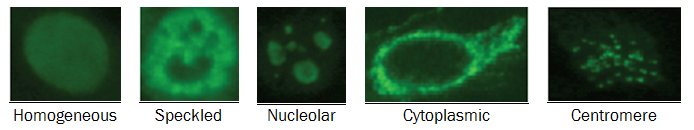
\includegraphics[scale=0.7]{Figures/introduction/cell_examples}
	\rule{35em}{0.5pt}
	\caption[Cell examples]{HEp-2 cell patterns}
	\label{fig:CellExamples}

\end{figure}

Although IIF posses qualities such as high sensitivity and a large number of antigens
that can be detected, it suffers from numerous shortcomings. The most important ones
are liability to subjectivity and time and labour consuming. \\

In order to avoid any kind of subjectivity , there is a great need for standardization and formalization of the mentioned procedure. Addressing this problem calls for CAD techniques which combines methods from machine learning and image analysis.

\section{Problem statement}

The content of the thesis proposes solutions for three major steps in the IFF process.

First of all, in order to find out a cell's pattern, cells should be isolated from an image aquired by IFF. As it is going to be explained (see chapter \ref{Chapter3}), although the problem of cell segmentation has been studied for more than 50 years, segmenting HEp-2 cells still suffers from certain problems, mostly due to different green flourescent protein apsorbtion accross the cells. This thesis proposes a method based on a region growing algorithm that demonstrates an encouraging result for overcoming mentioned problems. 

Once we have isolated the cells, the next step is to determine the fluorescent intensity of an image. The fluorescent intensity level can take three different values, namely \textit{positive}, \textit{intermediate} and \textit{negative}. A negative value means there are no observable cells in an image, while positive marks easily observable cells.  

The final step presents a novel approach to the staining pattern classification. The current state of the art solution solves the problem very succesfully, but acts like  black-box solutions not providing any explanation for the decision. This thesis tends to develop a method based on the human interpretable representation and reasoning. As IF-THEN rules are the most natural way of representing human knowledge,  the thesis will follow a rule mining approach, such as Inductive Logic Programming (ILP).
% Chapter Template

\chapter{Background} 

\label{Chapter2} % Change X to a consecutive number; for referencing this chapter elsewhere, use \ref{ChapterX}

%\lhead{Chapter 2. \emph{Understanding the domain}} % Change X to a consecutive number; this is for the header on each page - perhaps a shortened title

%----------------------------------------------------------------------------------------
%	SECTION 1
%----------------------------------------------------------------------------------------

\section{Understanding the domain}

\subsection{Immune system and antibodies }

The immune system is the central part of the human body responsible for protection against infections. In order to function properly, the immune system has to detect a wide range of threats, and at the same time distinguish them from  healthy tissue. The main weapon the immune system can use are antibodies.   \\

The antibody is a protein complex produced by \textit{B cells} \footnote{ a subgroup of white blood cells, a viral part of the immune system} that initiates an immune response against a target antigen \footnote{Foreign substance that, when introduced into the body, is capable of stimulating an immune response}. Their primal role is to recognize the unique part of the foreign target and  protect the body from infections. The basic organization of the antibody includes two functional domains that, together, resemble the letter Y (Figure \ref{fig:AntibodyIllustration}, left). The \textit{Fab}  part makes up the arms of the Y, and it contains the antigen-binding site - the region responsible for antigen binding. The \textit{Fc} part comprises the tail of the Y and effects other cells, proteins and antibodies.  \\

This unique structure allows detection of antigens, in direct or indirect manner. By direct detection we assume detection using a single fluorophore-labeled antibody, and by indirect detection we assume detection through binding of a fluorophore-labeled secondary antibody raised against the Fc part of an unlabeled primary antibody (as illustrated in Figure \ref{fig:AntibodyIllustration}, right). This system is versatile and cost-effective because few labeled antibodies are required to detect many possible primary antibodies. \\


\begin{figure}[htbp]
	\centering
	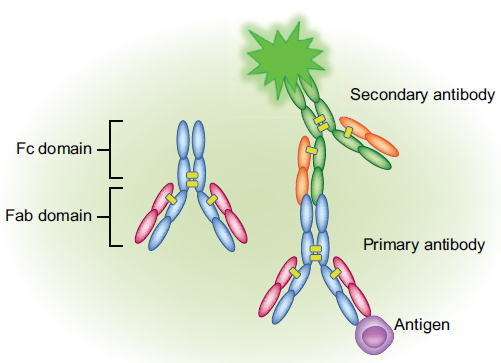
\includegraphics[scale=0.5]{Figures/Domain/antibodies}
	\rule{35em}{0.5pt}
	\caption[Illustration of antibody structure]{Illustration of antibody structure (from \cite{OdellCook2013})}
	\label{fig:AntibodyIllustration}

\end{figure}

The immune system can sometimes suffer from different disorders. A disorder of special importance to this Thesis is  \textit{autoimmunity}. Autoimmunity results in the disability of the immune system to recognize an organism's healthy tissue, and therefore attacks normal tissues as if they were foreign organisms. In the case of autoimmunity, antibodies are called antinuclear antibodies. We can observe those antibodies by using indirect immunofluorescence. \\

\subsection{Indirect Immunofluorescence}

As it was already mentioned, the indirect detection is the main focus of the thesis. Indirect immunofluorescence is a diagnostic methodology based on image analysis that reveals the presence of autoimmune diseases by searching for antibodies in the patient serum. Indirect immunofluorescence is a two-step technique, in which a primary, unlabeled antibody binds to the target, after which a fluorophore-labeled\footnote{fluorophore-labeling is a method to color the antibodies so they can be observed under the microscope} second antibody is used to detect the first antibody (figure \ref{fig:AntibodyIllustration}, right). Indirect immunofluorscence is more sensitive than a direct one because more than one secondary antibody can bind to each primary antibody, which amplifies the fluorescence signal. \\

As a result of its effectiveness,there has been a growing demand for diagnostic tests for systemic autoimmune diseases. Unfortunately,  IIF still remains a subjective method that depends too heavily on the experience and expertise of the physician. The main reasons causing the problems are:
\begin{itemize}
	\item the lack of quantitative information supplied to physicians
	\item varieties of reading systems and optics
	\item the photo-bleaching effect caused by a light source irradiating the cells over a short period of time
	\item the low reproducibility of the diagnostic protocol.
\end{itemize}

\subsection{Putting it all together}

The focus of this thesis is on the Antinuclear antibodies  test (ANA), which plays the main role in the serological\footnote{Further explanation} diagnosis of autoimmune disease. ANAs are directed against a variety of antigens and can be detected in patient serum through laboratory tests. IIF uses the human epithelial (HEp-2) substrate, which bonds with serum antibodies forming a molecular complex. This complex then reacts with human immunoglobulin \footnote{Immunoglobulin is a specific type of antibody created by plasma cells} and becomes visible under a fluorescence microscope which reveals the antigen-antibody reaction. \\

The procedure of ANA starts with  fluorescence intensity classification, a segmentation step is not a part of ANA procedure. The Center for Disease Control and Prevention in Atlanta,USA have published  guidelines \cite{nakamura1996quality} for scoring the intensity. The score ranges from 0 to 4+ as follows:
\begin{itemize}
	\item 4+ : brilliant green (maximal fluorescence)
	\item 3+ : less brilliant green fluorescence
	\item 2+ : defined pattern but diminished fluorescence
	\item 1+ : very subdued fluorescence
	\item 0 : negative.
\end{itemize}

Although the guidelines provide  very detailed instructions, in \cite{Rigon2007} Rigon et al. analyzed the variability between a set of physician's fluorescence intensity  classifications. Their work has shown a big variance of classifications made by physicians on the same dataset, so they suggested to classify the fluorescence intensity into three classes, namely negative, intermediate and positive. This work follows the protocol. \\

The final step consists of staining pattern recognition. As shown in figure \ref{fig:CellExamples}, there are several patterns that may be observed. \cite{FoggiaBenchmarks2013} and \cite{Perner02miningknowledge} provide a description of all staining patterns which is a valuable input taking into consideration a human interpretable perspective of this step. A summary is presented here:
\begin{itemize}

	\item \textbf{Centromere}: characterized by several discrete speckles ( $\sim$ 40 - 60) distributed throughout the interphase\footnote{The interphase is the nonmitotic phase of the cell cycle in which the cell spends the majority of its time and performs the majority of its purposes} nuclei and characteristically found in the condensed nuclear chromatin during mitosis as a bar of closely associated speckles.
	
	\item \textbf{Nucleolar}: characterized by clustered large granules in
the nucleoli of interphase cells which tend towards homogeneity, with less than six granules per cell.

	\item \textbf{Homogeneous}: characterized by a diffuse staining of the interphase nuclei and staining of the chromatin of mitotic cells.
	
	\item \textbf{Fine Speckled}: characterized by a fine granular nuclear staining of the interphase cell nuclei.
	
	\item \textbf{Coarse Speckled}: characterized by a coarse granular nuclear staining of the interphase cell nuclei.
	
	\item \textbf{Cytoplasmatic}: characterized by a highly irregular shape and large granule in the nucleoli

\end{itemize}


%------------------------------------------%
%                                          %
%           MACHINE LEARNING               %
%                                          %
%------------------------------------------%

\section{Machine learning}
% Chapter Template

\chapter{Literature overview} 

\label{Chapter3} % Change X to a consecutive number; for referencing this chapter elsewhere, use \ref{ChapterX}

%\lhead{Chapter 3. \emph{Literature overview}} % Change X to a consecutive number; this is for the header on each page - perhaps a shortened title

%----------------------------------------------------------------------------------------
%	SEGMENTATION
%----------------------------------------------------------------------------------------

\section{Cell segmentation}

Several studies have been proposed to classify autoantibody fluorescence patterns by using an automatic thresholding method, i.e.  Otsu's method, to segment the cells. The  thresholding method can choose the threshold to minimize the intraclass variance of the black and white pixels automatically. Due to the variety of ANA patterns,  Otsu's algorithm always failed to segment cells of speckled and nucleolar patterns, such as cases of a very blury image of low intensity. Figure \ref{fig:BadSegment} shows the over-segmentation results by using Otsu's algorithm. Additional challenge for the segmentation here is to separate overlapping cells which are quite common in the process.

\begin{figure}[htbp]
	\centering
	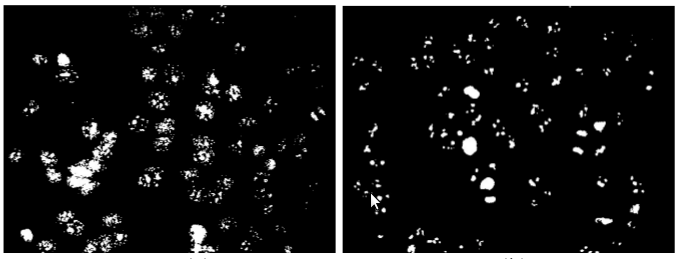
\includegraphics[scale=0.4]{Figures/introduction/badsegmentation}
	\rule{35em}{0.5pt}
	\caption[Bad segmentation example]{Segmentation results of the Otsu method (from \cite{Huang2008})}
	\label{fig:BadSegment}

\end{figure}


In \cite{Huang2008}, Huang et all. present an adaptive edged-based segmentation method for automatically detecting outlines of fluorescence cells in IIF images. Their approach is based on specific properties of the images regarding the pattern class. They have divided the images in two groups : sparse region and mass region cells. The mass region cells are those ones which have a \textit{compact} appearance, that look like a smooth object, while the sparse region cells are those ones for which we can detect multiple object in a cell. The approach trains a classifier to classify each image in the groups and applies different segmentation procedure for each group. In the case of the mass region cells, the cells are segmented using Otsu segmentation method, while in the case of the sparse region cell segmentation is performed by an edge detection. Their approach resulted in better segmentation results, but approximately 10\% of the cells remained undetected. \\

In \cite{HuangWatershed}, same authors further improve their method by incorporating watershed segmentation. The second approach also includes segmentation in two stages, depending on defined criteria. After a segmentation step performed by the watershed, the approach merges parts located relatively close and eliminates parts not large enough to represent a cell. If the retrieved number of regions doesn't safisfy the defined criteria, the segmentation step is performed again with different parameter settings determinated by Otsu's thresholding. \\

All forementioned approaches report similar shortcomings : approximately 10\% of cells remained undetected and the inability to separate overlapping cells.  The focus of the segmentation part of the Thesis will be on overcoming those problems. \\



%-----------------------------------------------------------------------------------------
%   INTENSITY LEVEL CLASSIFICATION
%-----------------------------------------------------------------------------------------

\section{Intesity level classification}

The following step, the intensity level classification, hasn't attracted a lot of scientific research, but has demonstrated remarkable results so far. \\

In \cite{SodaIntensity2006},  authors propose a system based on  \textit{Multi-Layer Perceptrons} and a \textit{Radial Basis Network} for the intensity classification step. That system, which makes use of features inspired from medical practice, shows error rates  up to 1\%, but it uses a reject option and it does not cast a result in about 50\% of cases. In \cite{SodaIntensity2009} the authors further refine their system. They train three experts, one specialized for each class, with a different set of features. They threat the classifiers similar to the \textit{one-vs-all} approach, so the final decision is made by a classifier most certain in it's decision. The authors report a success rate of 92,6\% accuracy. \\


%-----------------------------------------------------------------------------------------
%   STAINING PATTERN CLASSIFICATION
%-----------------------------------------------------------------------------------------

\section{Staining pattern classification}

As this problem was emphasized on the \textit{International Conference on Pattern Recognition 2012} as a contest, this step has been well researched and several very successful methods have been proposed. In \cite{FoggiaBenchmarks2013}, Foggia et al. provides a detailed overview of the methods submitted for the contest. The three most successful ones are presented here.  \\

In \cite{Kuan2012}, Kuan presents a method based on four texture descriptors: a rotation invariant form of local binary patterns (LBP) with multi-scale analysis,discrete cosine transformation, the mean values and standard variances of 2-D Gabor wavelets, and some global appearance based statistical features. A multiclass SVM was trained on each class of the four feature sets. The SVMs are then integrated in one classifier by using the AdaBoost.M1 algorithm. \\

In \cite{Nosaka2012}, Nosaka presents a similar approach on an extension of LBP, namely CoALBP \cite{Nosaka2011}. The advantage of this method is that the method can observe not only locals LBP, but also the spatial relations among adjacent LBP. The classifier is a linear SVM trained on an extended dataset including the rotated patterns of the original images. \\

Xianfeng et al. proposed a system based on MR8 method \cite{Varma2005} to extract statistical intensity features. The method calculates filter responses locally on the image, and then trains a global texton dictionary using $K$-means clustering. In that way, each image is represented by the frequency histogram of textons. The decision is made by a $k$-NN classifier. \\

Although there are many more papers in existance covering this problem, they are not presented here due to different, and not so rigorous, evaluation. Most of the early work was done on private datasets not available to public, which makes them not comparable to the new research results. Other papers with  a more recent date do not follow the evaluation procedure, so it is very hard to compare their efficiency with those ones in the overview. \\

More recently, a new overview of the method was presented by Agrawal et al. in \cite{Agrawal2013}. The committee of \textit{ICPR'13} has released a new, much bigger dataset for the same problem. The authors experimented with the most commonly used features in the previous contest - statistical features, histograms of oriented gradients, shape and size descriptors and texture descriptors. They have chosen the most typical representatives of classifiers, namely Naive Bayes, k-NN, SVM and Random forest. The SVM with Law's textural representation significantly  outperformed other classifiers and feature representations.



% ... and so on until
%\include{chap-n}
%\include{conclusion}

% If you have appendices:
\appendixpage*          % if wanted
\appendix
%% Chapter Template

\chapter{Research paper and code} % Main chapter title

\label{AppendixA} % Change X to a consecutive number; for referencing this chapter elsewhere, use \ref{ChapterX}

The code with the examples of usage can be found at \url{https://github.com/Sebac/MasterThesis_Code_final}.


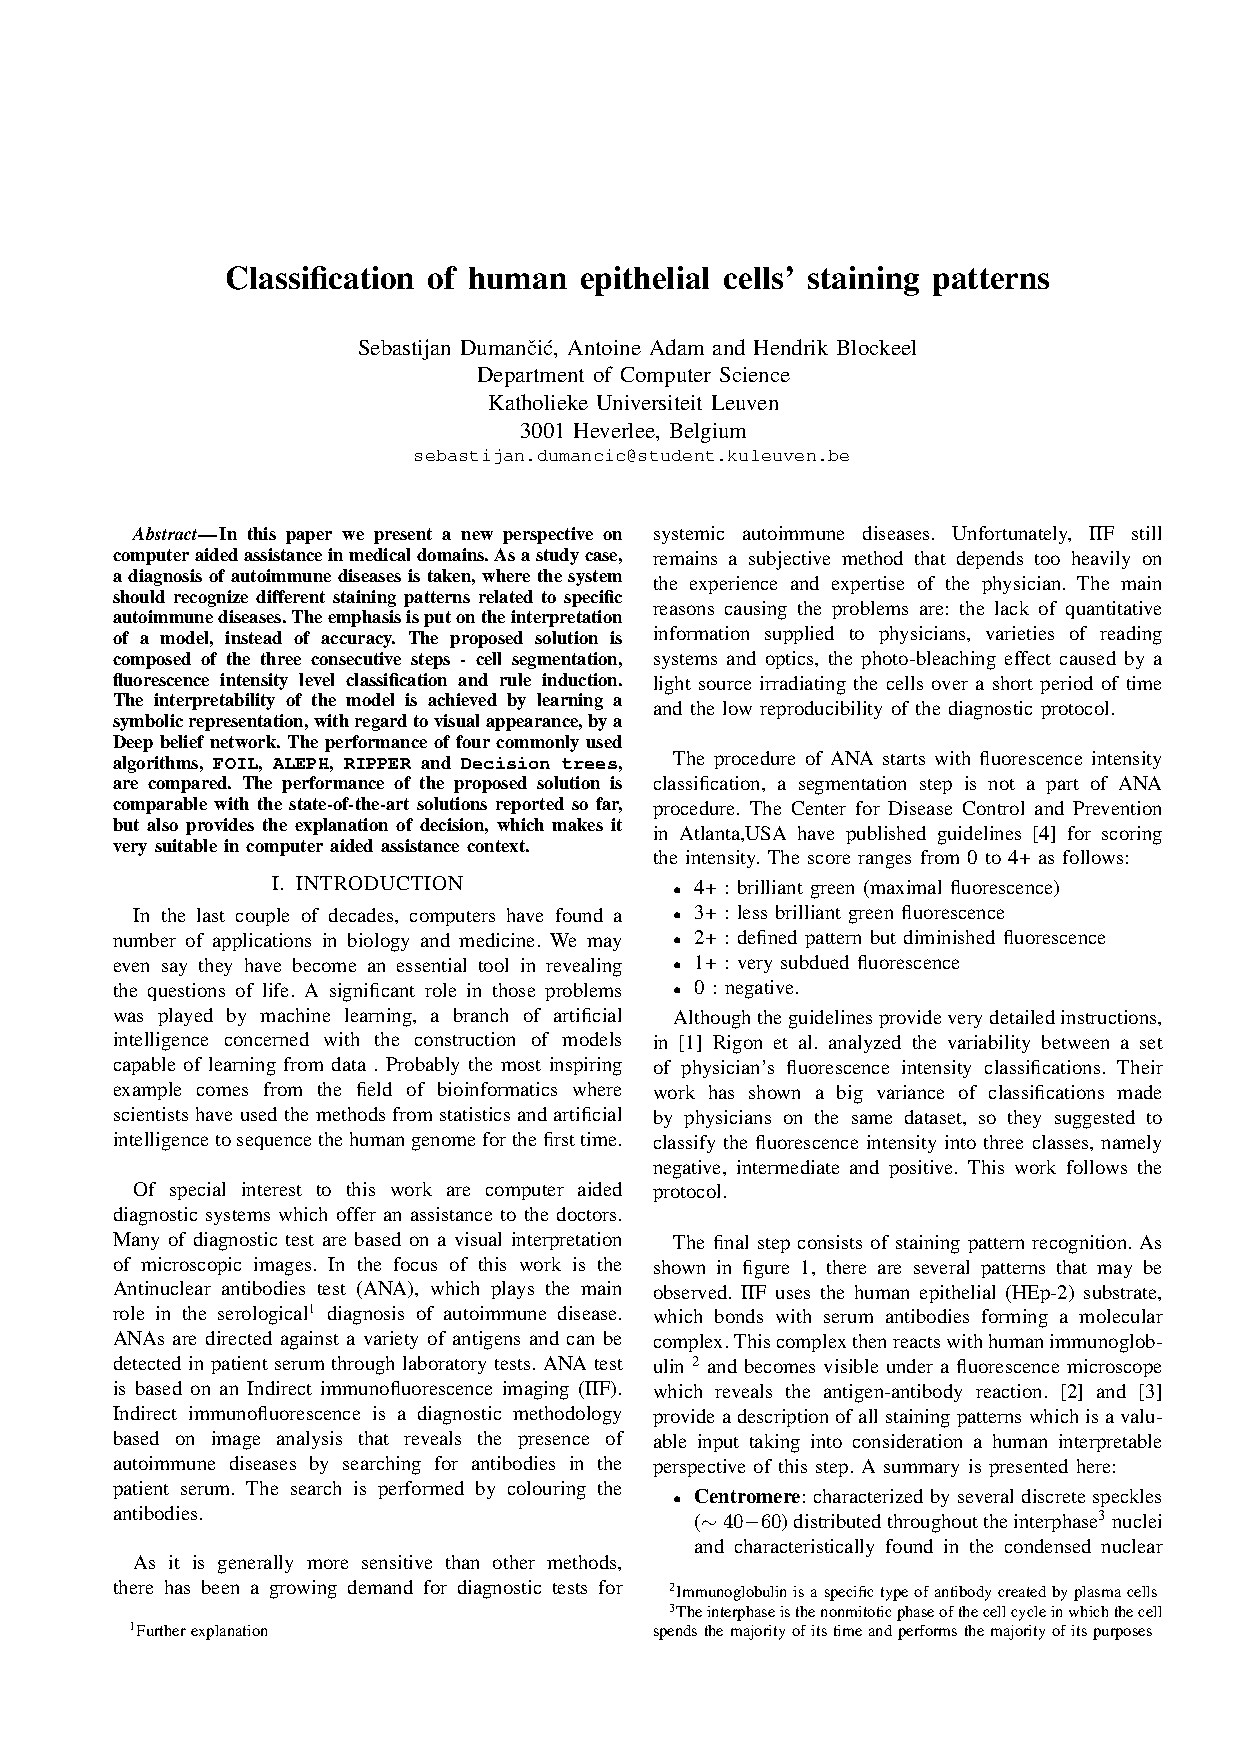
\includepdf[pages={1,2,3,4,5,6}]{../MasterThesis_paper/ieeeconf/paper.pdf}
% ... and so on until
%\include{app-n}

\backmatter
% The bibliography comes after the appendices.
% You can replace the standard "abbrv" bibliography style by another one.
\bibliographystyle{abbrv}
\bibliography{Bibliography}

\end{document}

%%% Local Variables: 
%%% mode: latex
%%% TeX-master: t
%%% End: 
